\chapter{Results}
\label{chap:results}

This chapter reports the outcomes of the evaluation protocol described in Section~\ref{sec:evaluation-methodology-full}, following the same order as the methodology chapter. Section~\ref{sec:regime-results} reports the regime-detection layer's validation results in full, since that layer's methodology (Sections~\ref{subsec:regime-engine-audit}--\ref{subsec:regime-synthetic-validation}) was substantially revised over the course of this project and its results directly informed how the layers built on top of it are interpreted. Section~\ref{sec:agent-results} reports a dedicated audit of the multi-agent deliberation layer (Section~\ref{sec:multi-agent-methodology}), tracing every agent from prompt to final action, followed by a prompt A/B test of regime context and a standalone five-asset backtest of the agents' consensus. Section~\ref{sec:rl-results} reports the RL execution layer's results (Section~\ref{sec:rl-execution-methodology}): a controlled ablation on the crypto-only panel that produced this project's final decision on that layer, and a weekly-decision-cadence follow-up whose initially promising result did not replicate out of sample.

\section{Regime Detection Results}
\label{sec:regime-results}

Six regime-detection configurations were carried through the full validation battery: the original four-asset, encoder-based production model; the five-asset crypto-only panel introduced in Section~\ref{subsec:regime-asset-panel-revision}, in both its 14-column production-feature form and a 22-column form extended with 90-day and 180-day rolling-normalization horizons alongside the production 720-hour window; and the same two feature variants restricted to BTC alone, retained throughout as a single-asset comparison baseline.

\subsection{Statistical Validity Across Candidate Configurations}
\label{subsec:regime-results-preview}

\begin{table}[H]
\centering
\small
\caption{Seed stability and distinctness across all six configurations tested. Seed ARI is the mean pairwise Adjusted Rand Index across five independent EM restarts (Section~\ref{subsec:regime-engine-audit}). \texttt{close\_return} / \texttt{realized\_vol\_raw} distinctness report the outcome of a per-asset ANOVA across states on that quantity.}
\label{tab:regime-six-model-distinctness}
\begin{tabular}{|l|c|c|p{3.9cm}|c|}
\hline
\textbf{Configuration} & \textbf{States} & \textbf{Seed ARI} & \textbf{\texttt{close\_return} distinctness} & \textbf{\texttt{realized\_vol\_raw}} \\
\hline
Production (4-asset) & 4 & 0.193 & weak, 1--3/6 pairs indistinguishable per asset & $p\approx0$, all \\
\hline
5-asset, 14-col & 6 & 0.585 & 4/5 assets significant, 0 indistinguishable pairs & $p\approx0$, all \\
\hline
5-asset, 22-col & 6 & \textbf{1.000} & 2/5 assets significant, 0 indistinguishable pairs & $p\approx0$, all \\
\hline
BTC-only, 14-col & 6 & 0.698 & not significant, 0 indistinguishable pairs & $p\approx0$ \\
\hline
BTC-only, 22-col & 6 & \textbf{0.989} & not significant, 0 indistinguishable pairs & $p\approx0$ \\
\hline
\end{tabular}
\normalsize
\end{table}

\begin{table}[H]
\centering
\small
\caption{Next-hour directional predictive signal (AUC, logistic regression, walk-forward test split) for the same six configurations.}
\label{tab:regime-six-model-auc}
\begin{tabular}{|l|c|c|}
\hline
\textbf{Configuration} & \textbf{regime\_only AUC} & \textbf{features\_only AUC} \\
\hline
Production (4-asset) & 0.489--0.505 & 0.506--0.544 \\
\hline
5-asset, 14-col & 0.498--0.523 & 0.528--0.548 \\
\hline
5-asset, 22-col & 0.503--0.521 & 0.528--0.548 \\
\hline
BTC-only, 14-col & 0.494 & 0.542 \\
\hline
BTC-only, 22-col & 0.501 & 0.542 \\
\hline
\end{tabular}
\normalsize
\end{table}

Two findings hold across all six configurations without a single exception. Volatility distinctness (\texttt{realized\_vol\_raw}, ANOVA across states, tested per asset independently) is significant at $p\approx0$ in every configuration and every asset --- the discovered states are genuine, statistically real volatility clusters regardless of panel or feature-horizon choice. Next-hour directional predictive signal from the regime label alone is chance-level (AUC 0.49--0.52) in every configuration, and adding the regime label on top of the raw features never measurably improves on the raw features alone.

A trade-off not visible from either extreme alone emerged once every feature-horizon variant had been tested against the same battery: the 22-column feature set gives near-perfect seed stability (0.989--1.000) at the cost of weaker return distinctness (2/5 assets significant versus 4/5 for the 14-column set on the five-asset panel), and neither variant's return-distinctness advantage translates into predictive AUC. The 22-column set is preferred for anything requiring a reproducible regime definition across refits, on the reasoning that a return-distinctness advantage that does not translate into predictive signal is worth less than reproducibility, but this is a judgment call between two real, opposing properties rather than a configuration that dominates on every axis.

\subsection{Regime Characterization}
\label{subsec:regime-characterization}

Table~\ref{tab:regime-characterization} reports the fitted per-state statistics for the six-state, five-asset, 22-column configuration --- the production regime model referenced throughout the remainder of this chapter and used by both the multi-agent and RL layers. Labels are generated automatically from each state's $\overline{\mathrm{realized\_vol}}$ (bucketed into five volatility tiers) and the sign of $\overline{\mathrm{adx}}$ (trending versus range-bound), the same direction-agnostic classifier documented in Section~\ref{subsec:regime-label-fix}; no directional (``bull''/``bear''/``crisis'') language is used, for the reasons Section~\ref{subsec:regime-zigzag} establishes below.

\begin{table}[H]
\centering
\small
\setlength{\tabcolsep}{4.5pt}
\renewcommand{\arraystretch}{1.3}
\caption{Per-regime fitted statistics, six-state five-asset 22-column configuration (pooled 2018--2025 training data). Sharpe, annualized return, and annualized volatility are historical population averages conditional on regime membership, not forward-looking predictions --- see Section~\ref{subsec:regime-zigzag}.}
\label{tab:regime-characterization}
\begin{tabular}{|c|p{3.3cm}|c|c|c|c|c|}
\hline
\textbf{Regime} & \textbf{Label} & \textbf{Sharpe} & \textbf{Return} & \textbf{Vol} & \textbf{Share} & \textbf{Asset} \\
\hline
R0 & Very Low Volatility / Range-bound & $-1.04$ & $-34.8\%$ & $33.5\%$ & $15.2\%$ & BTC \\
\hline
R1 & Moderate Volatility / Trending & $+1.11$ & $+74.4\%$ & $67.0\%$ & $17.2\%$ & LTC \\
\hline
R2 & Low Volatility / Range-bound & $-0.22$ & $-14.7\%$ & $68.3\%$ & $18.8\%$ & ETH \\
\hline
R3 & Low Volatility / Range-bound & $-0.26$ & $-12.4\%$ & $46.9\%$ & $20.3\%$ & XRP \\
\hline
R4 & Elevated Volatility / Trending & $+1.39$ & $+140.6\%$ & $101.5\%$ & $19.4\%$ & ETH \\
\hline
R5 & Extreme Volatility / Trending & $-0.44$ & $-82.7\%$ & $189.8\%$ & $9.0\%$ & XRP \\
\hline
\end{tabular}
\renewcommand{\arraystretch}{1.0}
\normalsize
\end{table}

\begin{figure}[!htbp]
    \centering
    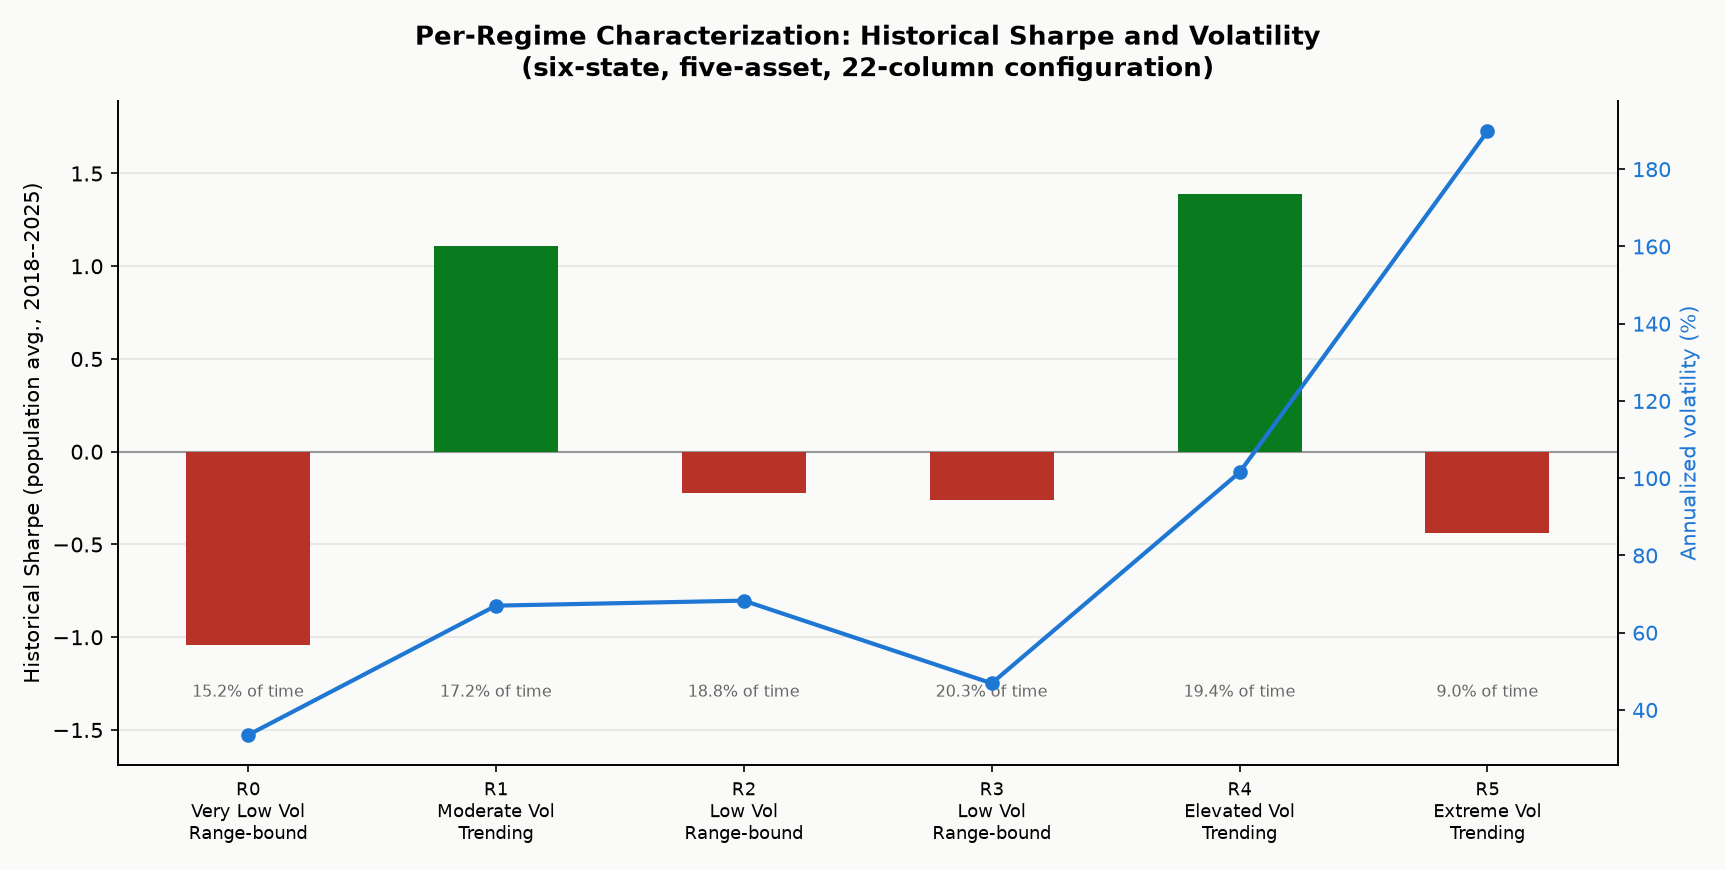
\includegraphics[width=\textwidth]{images/regime_characterization_barplot.png}
    \caption{Per-regime historical Sharpe (bars, left axis) and annualized volatility (line, right axis), six-state five-asset 22-column configuration. Time-share annotations below each bar show the fraction of pooled 2018--2025 hours spent in that regime.}
    \label{fig:regime-characterization}
\end{figure}

Read purely as descriptive statistics, R0 and R5 resemble a natural short-or-avoid signal and R4 a natural long signal. Section~\ref{subsec:regime-zigzag} tests this reading directly at the level of individual price legs rather than accepting it at face value, and finds that it does not hold: these historical averages describe each state's unconditional population history over 2018--2025, not a leg-by-leg or forward-looking predictive property, and R4 in particular is dominant on \emph{more} down-legs than up-legs despite carrying the highest historical Sharpe of any state.

\subsection{Downstream Value: Position Sizing and Directional Conditioning}
\label{subsec:regime-downstream-value}

Two self-contained backtest designs --- deliberately excluding the RL execution and multi-agent layers of Sections~\ref{sec:multi-agent-methodology}--\ref{sec:rl-execution-methodology}, so that the regime signal's standalone value could be isolated from anything a learned policy might extract from it --- were run on the walk-forward validation (2024) and test (2025) splits of the five-asset panel, using the 22-column configuration: regime-conditioned position sizing (Table~\ref{tab:regime-sizing-backtest}) and regime-gated directional trading with a noise control (Table~\ref{tab:regime-directional-backtest}).

\begin{table}[H]
\centering
\small
\caption{Regime-conditioned volatility-target position sizing versus buy-and-hold and continuous (regime-free) volatility targeting, five-asset equal-weight portfolio.}
\label{tab:regime-sizing-backtest}
\begin{tabular}{|l|c|c|c|}
\hline
\textbf{Split} & \textbf{buy\_hold} & \textbf{vol\_target (continuous)} & \textbf{regime\_conditioned} \\
\hline
2024 (validation) & \textbf{+1.203} & +0.353 & +0.386 \\
\hline
2025 (test) & \textbf{--0.131} & --0.343 & --0.364 \\
\hline
\end{tabular}
\normalsize
\end{table}

Buy-and-hold outperformed both sizing strategies in both periods, and regime-conditioned sizing was never significantly different from continuous, regime-free volatility targeting (block-bootstrap 95\% confidence interval on the Sharpe delta, 1000 resamples over non-overlapping 168-hour blocks, crosses zero in both 2024 and 2025). Discretizing volatility into HMM regime buckets did not outperform simply dividing by trailing realized volatility directly for this sizing rule.

A second design tested whether regime could instead gate \emph{when to trust} a directional signal, rather than only scale an always-long position: a 24-hour momentum rule (long or short by the sign of the trailing 24-hour return) was combined with a gate that permitted a position only when the current state had shown a positive Sharpe ratio for that same rule on training data, with the gate threshold decided from training data only in every case. A first pass, without a control, found this gate improving the momentum rule's Sharpe by roughly one full point in both periods (95\% CI $[0.119, 2.094]$ in 2024, significant). A noise-control arm was then added --- an independently simulated Markov chain using the real fitted transition matrix, giving it identical persistence and gating frequency to the real regime label while carrying zero actual information about the asset's price path --- and this changed the conclusion materially:

\begin{table}[H]
\centering
\small
\caption{Directional gating: real regime versus a matched noise control, momentum strategy, five-asset portfolio.}
\label{tab:regime-directional-backtest}
\begin{tabular}{|l|c|c|c|}
\hline
\textbf{Split} & \textbf{momentum\_only} & \textbf{regime-gated} & \textbf{noise-gated} \\
\hline
2024 (validation) & --2.619 & --1.488 & \textbf{--1.050} \\
\hline
2025 (test) & --2.863 & --1.998 & --2.750 \\
\hline
\end{tabular}
\normalsize
\end{table}

In 2024, the noise-gated control performed as well as, and by point estimate slightly better than, the real regime gate (regime-versus-noise 95\% CI $[-1.721, 0.984]$, not significant), while both were significantly better than no gating at all. The underlying momentum rule is deeply unprofitable on its own (Sharpe $-2.6$ to $-2.9$ in both periods), and any gate that reduces net exposure to a structurally losing strategy mechanically improves its Sharpe ratio whether or not the gate carries genuine information --- which is what the noise control demonstrates directly rather than leaving as a theoretical concern. 2025 shows a larger gap favoring the real regime gate (regime-versus-momentum CI $[-0.209, 2.162]$; noise-versus-momentum CI $[-1.134, 1.25]$), but neither period shows the real gate beating the noise control at conventional significance. Across both backtest designs, standalone regime conditioning did not demonstrate a measurable, noise-control-surviving improvement in risk-adjusted return.

\subsection{Regime Label Directional Fidelity: A Leg-Level Check}
\label{subsec:regime-zigzag}

The backtests above ask whether regime conditioning adds measurable value to a trading rule. A more basic question, prior to any trading rule, is whether a regime's own name describes what it actually does: does a state labeled ``bull'' predominate during genuine price advances, and a state labeled ``bear''/``crisis'' during genuine declines? This was tested directly with a standard zigzag/peak-trough segmentation (a $\geq$15\% threshold move, an objective, data-determined criterion, not tuned to the outcome) applied to daily close price for all five crypto5-panel assets over 2021 --- a year containing both the panel's largest rally and one of its sharpest corrections. Each resulting leg (111 total across the five assets) was assigned the \emph{dominant} (mode) regime label over its duration, and that label's class (bull-labeled, bear-labeled, or crisis) was checked against the leg's actual direction.

\begin{table}[H]
\centering
\small
\caption{Regime-label dominance by leg direction, five-asset panel, 2021 (111 legs total, zigzag threshold 15\%).}
\label{tab:regime-zigzag}
\begin{tabular}{|l|l|c|c|c|}
\hline
\textbf{Regime} & \textbf{Label} & \textbf{Up-legs} & \textbf{Down-legs} & \textbf{\% up} \\
\hline
R0 & bear / drawdown & 1 & 4 & 20\% \\
\hline
R1 & mild bull & 6 & 3 & 67\% \\
\hline
R2 & mild bear / chop & 21 & 17 & 55\% \\
\hline
R3 & low-vol bear & 7 & 8 & 47\% \\
\hline
R4 & strong bull & 13 & 19 & 41\% \\
\hline
R5 & crisis & 6 & 6 & 50\% \\
\hline
\end{tabular}
\normalsize
\end{table}

Overall match rate: \textbf{54/111 (48.6\%)} --- statistically indistinguishable from a coin flip. R0 and R1 show a genuine directional lean; R2 through R5 do not, and R4 --- the state literally labeled \emph{strong bull} --- is dominant more often on down-legs than up-legs. This is not a rare miscall: two consecutive, unambiguous legs in the BTC series alone illustrate it directly. A $-25.2\%$ decline from 2021-01-08 to 2021-01-27 was dominated (52.5\% of its hours) by R4; the very next leg, an $+89.1\%$ advance from 2021-01-27 to 2021-02-21, was dominated (67.0\%) by R2, ``mild bear/chop.''

The cause is visible directly in the regime's own fitted feature means (Section~\ref{subsec:regime-final-fit}): R4 has $\overline{\mathrm{rsi}} \approx -0.005$ (direction-neutral) but $\overline{\mathrm{realized\_vol}} = +0.74$ and $\overline{\mathrm{adx}} = +0.24$ (both clearly elevated) --- R4 is not a bullish cluster, it is a \emph{high-volatility, strongly-trending} cluster that fires on trend strength regardless of sign. Its historical Sharpe of $+1.39$, the statistic its name is derived from, is a population average over 2018--2025, a period in which crypto had more net-bullish high-volatility-trending hours than net-bearish ones; it describes the state's unconditional history, not a leg-by-leg predictive property, and is misleading if read as a forward-looking directional signal. This is consistent with, and considerably sharper than, every other finding in this section: the states are genuine volatility/trend-magnitude clusters (Section~\ref{subsec:regime-results-preview}'s distinctness result), not directional predictors, and their plain-language names should not be read as one.

\subsection{Consequence: Removing Directional Language from Regime Descriptions}
\label{subsec:regime-label-fix}

The zigzag result above is not only descriptive: the same Sharpe-derived bull/bear/crisis text it discredits was originally the literal string shown in the dashboard's regime legend and injected into every LLM agent's prompt as the qualitative description of current market conditions --- exactly the kind of directional-sounding label the leg-level check just showed does not reliably correspond to actual price direction. This was corrected directly: a volatility/trend-strength classifier (built from $\overline{\mathrm{realized\_vol}}$ and $\overline{\mathrm{adx}}$, both direction-agnostic by construction --- ADX measures trend strength regardless of sign in standard technical analysis) replaced the sharpe-derived bucketing in four places: the crypto5 production description generator and the legacy EURUSD/GOLD description generator in the dashboard backend (the latter fixed for consistency with the same anti-pattern, though not independently re-validated with an equivalent forex zigzag test), the static fallback dictionary, and --- the change with actual behavioral reach --- the description builder in the multi-agent context module (Section~\ref{subsec:regime-context}), which supplies the text every LLM agent reads as market character. A previously disconnected, hardcoded legend in the dashboard frontend was also wired to the same live source instead of a stale duplicate. For example, what previously read \emph{``Elevated Volatility / Strong Bull''} for R4 now reads \emph{``Elevated Volatility / Trending''}. The full regime-quality audit (Sections~\ref{subsec:regime-results-preview}, \ref{subsec:regime-synthetic-results}) was re-run afterward and confirmed byte-identical to its pre-fix output on every statistical section, since only description text was changed, not the underlying HMM decode.

\textbf{The same directional assumption also existed in trading logic: the separate Sharpe-bucketed classifier feeding \texttt{FundManagerAgent}'s conviction multipliers} (Section~\ref{subsec:fund-manager-synthesis}) encoded the same directional assumption the zigzag test discredited --- concretely, a bullish consensus occurring during R5 (crisis, empirically 50/50 directional) was unconditionally overridden to \texttt{hold} regardless of what the debate concluded, and R4 (empirically more down-legs than up-legs) carried a bullish-favoring conviction multiplier. Unlike the description fix above, this is trading logic rather than display text, so it was addressed as a separate, explicit change rather than folded into the same pass: the sharpe-sign classifier and its bullish/bearish penalty and override sets were removed, and conviction is now scaled by \texttt{classify\_regime\_volatility\_level} --- the same \texttt{realized\_vol\_mean}-derived, direction-agnostic dimension validated above --- symmetrically for bullish and bearish calls, with no action-forcing override tied to an assumed direction. Verified directly: a bullish consensus during R5, which previously forced \texttt{final\_action="hold"} irrespective of the debate's actual conclusion, now correctly returns \texttt{"long"} at reduced conviction (0.6$\times$, reflecting R5's genuinely elevated volatility, not an assumed direction); R4 now scales bullish and bearish conviction identically (0.8$\times$ each) rather than favoring bullish. The trade-off is explicit: R0 and R1, the two regimes the zigzag test found to carry a real (if modest) directional lean, no longer receive any directional weighting either, since \texttt{classify\_regime\_kind} could not distinguish their validated lean from R2/R3/R4's discredited one without reverting to a per-regime-index table (rejected earlier in this project for going stale on every HMM refit). Full regression suite (50 tests across the agent and observation-builder test modules) passes unchanged after this edit.

\subsection{Synthetic Recovery Summary}
\label{subsec:regime-synthetic-results}

\begin{table}[H]
\centering
\small
\caption{Synthetic ground-truth recovery (Adjusted Rand Index) across every mechanism tested (Section~\ref{subsec:regime-synthetic-validation}).}
\label{tab:regime-synthetic-results}
\begin{tabular}{|l|c|}
\hline
\textbf{Configuration} & \textbf{ARI} \\
\hline
Single asset, 1 year, single seed & 0.166 \\
\hline
Single asset, 3 years, single seed & 0.167 \\
\hline
Single asset, 1 year, best-of-5-seed production procedure & 0.156 \\
\hline
5 independent synthetic assets pooled, 1 year each & 0.163 \\
\hline
5 correlated synthetic assets pooled (96\% simultaneous co-movement) & 0.176 \\
\hline
5 assets pooled at production's real scale ($\approx$246{,}000 rows) & 0.162 \\
\hline
\hline
Bayes-optimal classifier, true parameters, no estimation & \textbf{0.047} \\
\hline
\end{tabular}
\normalsize
\end{table}

No mechanism tested moved recovery accuracy outside a narrow 0.15--0.20 band, including the configuration built to match production's real data scale and asset count directly, and the Bayes-optimal ceiling computed from the true generating parameters sits below every empirically achieved value in the table --- confirming, as discussed in Section~\ref{subsec:regime-synthetic-validation}, that recovery accuracy at this task is bounded by genuine overlap between the six states' return distributions rather than by anything the estimation pipeline could be expected to improve with more data.

\section{Multi-Agent Deliberation Results}
\label{sec:agent-results}

The multi-agent layer (Section~\ref{sec:multi-agent-methodology}) was audited end to end --- prompt to final action, twenty real Mistral~7B calls, \texttt{BTC\_USDT} at 2024-03-01, three purpose-built validation tests (Table~\ref{tab:agent-validation-battery}) followed by targeted adversarial checks --- rather than assumed to behave as its architecture description implies. The audit's central finding reframes the system's own description: it is not ``multi-agent debate decides trades.'' Three agents (Macro, Technical, Sentiment) supply LLM-sourced directional opinions; the Contrarian's dissenting direction is forced in code, not decided by its own model call; one agent (Risk) never calls an LLM at all; and the Fund Manager's actual decision --- action, position size, conviction, dissent list --- is deterministic arithmetic over the other agents' outputs, with its one LLM call producing only the rationale sentence, never the decision itself. The system is better described as a deterministic, risk-weighted consensus engine with LLM-assisted directional inputs.

\subsection{Validation Battery: What the System Actually Does}
\label{subsec:agent-validation-battery}

\begin{table}[H]
\centering
\small
\setlength{\tabcolsep}{4.5pt}
\renewcommand{\arraystretch}{1.3}
\caption{Multi-agent layer validation battery (20 real Mistral 7B calls, \texttt{BTC\_USDT} 2024-03-01).}
\label{tab:agent-validation-battery}
\begin{tabular}{|p{3.2cm}|p{6.0cm}|p{3.3cm}|}
\hline
\textbf{Test} & \textbf{What it checks} & \textbf{Result} \\
\hline
Schema & Every call returns a valid, non-fallback response & 6/6 agents pass \\
\hline
Null-regime & Swapping the real regime for a random one measurably changes output & 3/3 directional agents pass \\
\hline
Aggregator-usage & Flipping one agent's thesis (no new LLM call) changes the Fund Manager's conviction and dissent list & Pass (0.81 $\to$ 0.51 conviction shift observed) \\
\hline
\end{tabular}
\renewcommand{\arraystretch}{1.0}
\normalsize
\end{table}

The null-regime test confirms regime context is not silently discarded by the directional agents, and the aggregator-usage test confirms the deterministic vote genuinely reads every agent's output rather than hardcoding an answer --- both properties that the architecture description alone would not establish.

\subsection{Failure Modes Found, and Their Resolution}
\label{subsec:agent-failure-modes}

\textbf{TechnicalAgent ignored obvious bearish price action; fixed and verified.} On an adversarial case (RSI 12, strongly negative MACD, $-6\%$ return), the agent reported ``bullish, confidence 0.65,'' reasoning that the regime's qualitative description text (``high-volatility bull regime'') supported a rebound. An ablation isolating the cause --- rather than assuming weak reasoning in general --- found the loaded ``bull''/``bear'' wording in the regime description text acting as a dominant lexical anchor for the 7B model: with that text present, 0/3 repeated runs on the adversarial case got the direction right; neutralizing the regime description entirely reached 1/3; stripping only the loaded wording while keeping the real regime label and probability vector (already confirmed informative by the null-regime test) reached 4/5. The fix builds the Technical agent's prompt from a context copy with the regime description replaced by a neutral placeholder, adds explicit ADX-conditioned interpretation rules for extreme RSI/MACD readings, and exposes \texttt{close\_return} explicitly (previously silently truncated from the shared price-features block). Verified 5/5 correct on both bearish and bullish extremes post-fix, with the real, unmodified 2024-03-01 context re-checked to confirm normal-case output is unchanged.

\textbf{Regime sensitivity is real but was initially not cleanly directional; this did not reproduce on the crypto-only panel.} Forcing the Macro agent's regime block to the single best-Sharpe regime in the original four-asset dataset did not make it more bullish --- output collapsed to neutral/0.50, the same response every synthetic regime (bull, bear, sideways, random) produced; only the \emph{actual} regime, which happened to agree with the agent's own correlation data, produced a confident call. Re-running the identical synthetic-regime methodology after the migration to the five-asset crypto-only panel (Section~\ref{subsec:regime-asset-panel-revision}) did not reproduce this collapse: the Macro agent scored 2/2 bullish on the bull variant, 2/2 bearish on the bear variant, and 2/2 neutral on the sideways variant. The Sentiment agent showed a milder version of the original inconsistency (1/2 bearish on the bear variant). Why the original finding no longer holds is not established --- plausibly the crypto-only panel's regime descriptions carry more distinguishing information, plausibly the effect was always closer to the edge of reproducibility than the original characterization implied.

\textbf{ContrarianAgent's dissent is intentionally not LLM-generated.} Its \texttt{directional\_bias} is forced to the opposite of consensus in code regardless of the model's own output; only confidence, reasoning, and key factors come from the model. This is a deliberate design choice --- guaranteeing opposition for the Fund Manager to weigh --- not a discovered defect, and is stated here so the system is not described as ``a debating agent'' without the caveat.

\textbf{RiskAgent instantiates an LLM client it never calls.} Harmless in practice (its GARCH-based volatility forecast and CVaR position caps are pure computation, Section~\ref{subsec:risk-agent-detail}), but worth correcting in any architecture diagram that implies otherwise.

\textbf{Regime staleness could silently reach the prompt; fixed.} The regime-context builder could serve a regime row up to twenty hours old on a data gap with no signal to the agent or the prompt. Fixed with an explicit staleness flag and gap-hours field, surfaced in the prompt when triggered; verified against both an exact-match timestamp (not flagged) and a known 20-hour gap (correctly flagged).

\textbf{ContrarianAgent JSON parse failures had the wrong root cause identified initially.} A prior hypothesis attributed roughly 40\% of parse failures to output truncation at the token generation cap. A controlled repro found instead that all three test calls produced complete, well-formed JSON, and the actual failure was schema validation rejecting a reasoning field that exceeded its maximum length --- the one prompt among the five agents' that never instructed the model to keep its answer short. Fixed by adding an explicit length instruction to the prompt and adding a schema-generic recovery stage that clips any oversized field to its declared constraint via the schema's own field metadata, covering the same failure class for any other agent's field, not only this one.

\textbf{Migration and regression verification.} Following the panel migration (Section~\ref{subsec:regime-asset-panel-revision}), five real end-to-end debates (unmocked LLM calls) were run, one per crypto-panel asset, including three assets with no prior debate coverage. All five completed successfully; the Contrarian agent returned real historical-analogue evidence (31--66\% historical loss rates) for every asset rather than the silent empty result it previously returned for the three newly added assets; the Risk agent produced five distinct real GARCH volatility forecasts; and the Macro agent's correlation matrix covered all ten asset pairs. Full regression after this and the parsing fix above: 83 of 83 tests passing in the affected suites, with four pre-existing failures elsewhere in the repository (dashboard API and RL-environment dimension drift) confirmed present before this work began and unrelated to it.

\subsection{Regime Context in the Prompt: an A/B Test}
\label{subsec:agent-instructions-ab}

The null-regime test shows that regime context changes agent output; it does not show whether that change is useful. A pre-registered A/B/C test ran the same (timestamp, asset) pairs through three prompt variants: \emph{none} (no regime context), \emph{description\_only} (the production prompt, describing the current regime), and \emph{instructions} (the description plus explicit risk rules, e.g.\ ``max 30\% of normal risk budget'' in extreme volatility). Timestamps were stratified by volatility level (10 per level and variant, 90 debates in total, all before 2025 so the test split was not touched). With 8--10 directional calls per cell, no bootstrap interval was computed; the results below are a consistent pattern across four metrics, not a significance-tested finding.

\begin{table}[H]
\centering
\small
\caption{Regime-context prompt A/B test (90 real debates, $n=30$ per variant, pre-2025 timestamps). Position, conviction, and agreement are means over the variant's debates.}
\label{tab:agent-instructions-ab}
\begin{tabular}{|l|c|c|c|c|}
\hline
\textbf{Variant} & \textbf{Dir.\ acc.} & \textbf{Position} & \textbf{Conviction} & \textbf{Agreement} \\
\hline
none & 0.556 (15/27) & 0.377 & 0.536 & 0.678 \\
\hline
description\_only & 0.571 (16/28) & 0.477 & 0.644 & 0.731 \\
\hline
instructions & 0.552 (16/29) & 0.508 & 0.691 & 0.783 \\
\hline
\end{tabular}
\normalsize
\end{table}

Directional accuracy is the same for all three variants (0.55--0.57). The hypothesis that explicit risk instructions would \emph{reduce} position size in high-volatility regimes was not just unsupported but inverted: position size, conviction, Round-2 flip rate, and agent agreement all rise with the amount of regime text in the prompt, in every volatility level, and the largest extreme-volatility position (0.350) came from the \emph{instructions} variant. The cause is architectural: position size is computed in code from conviction (Section~\ref{subsec:fund-manager-synthesis}), and a sizing rule written in the prompt is text the agents read, not a constraint anything enforces. The rule was therefore moved into code as a hard volatility-level ceiling on position size (Section~\ref{subsec:fund-manager-synthesis}); a deterministic check confirmed that a maximum-confidence case in extreme volatility, previously sized at 0.48, is now capped at 0.30, while normal-volatility decisions are unchanged. This check verifies the code path; the 90-debate test was not re-run with the cap in place.

\subsection{Standalone Trading Backtest of the Agent Layer}
\label{subsec:agent-standalone-backtest}

To measure the agent layer's own trading value, independently of the RL layer, its consensus was run as a rule on all five crypto5 assets over the 2024 validation year: at every hour, the nearest cached debate within seven days sets the direction and the (risk-capped) position size, with no PPO involved. This required real debate coverage for every asset; a batch generation pass produced about 366 daily-stride debates per asset over 2024 (1{,}855 debates in total). Every debate was generated with the full regime context in its prompts, so this test measures the regime-conditioned agent layer against buy-and-hold; no regime-free set of debates exists to isolate the regime's own contribution.

\begin{table}[H]
\centering
\small
\caption{Agent consensus rule versus buy-and-hold, 2024 validation, per asset. $\Delta$ Sharpe with 95\% block-bootstrap CI (1000 resamples).}
\label{tab:agent-standalone-backtest}
\begin{tabular}{|l|c|c|c|c|c|}
\hline
\textbf{Asset} & \textbf{Buy-hold Sharpe} & \textbf{Agents Sharpe} & \textbf{$\Delta$ Sharpe} & \textbf{95\% CI} & \textbf{Sig.} \\
\hline
BTC & 1.498 & 1.088 & $-0.381$ & $[-2.27, +1.54]$ & no \\
\hline
ETH & 0.583 & 1.192 & $+0.553$ & $[-1.42, +2.69]$ & no \\
\hline
BNB & 1.287 & 3.214 & $+1.944$ & $[+0.09, +3.83]$ & yes \\
\hline
LTC & 0.427 & 2.787 & $+2.445$ & $[+0.14, +4.95]$ & yes \\
\hline
XRP & 1.346 & 0.402 & $-0.880$ & $[-3.57, +1.92]$ & no \\
\hline
\end{tabular}
\normalsize
\end{table}

Two of five assets (BNB, LTC) show a significantly higher Sharpe ratio than buy-and-hold; three do not. This should not be read as a directional edge. The agents rule takes small, tightly capped positions (about 200--240 meaningful trades per asset, 1.1--2.9\% maximum drawdown, 2.7--10.1\% total return), whereas buy-and-hold carries full exposure (36--58\% maximum drawdown). The two significant cases are largely explained by buy-and-hold being unusually poor on a risk-adjusted basis for those assets (for LTC, $+1.8\%$ return against a 57.8\% drawdown). Moreover, with five independent tests at the 95\% level, about one false positive is expected even if no effect exists \cite{harvey2016}; two of five is suggestive, not conclusive.

\subsection{Relationship to the Reported RL Policy}
\label{subsec:agent-rl-disconnect}

The debate system is never invoked during RL training or evaluation (Section~\ref{sec:rl-execution-methodology}). The checkpoints behind the RL results in Section~\ref{sec:rl-results} use raw-feature observation modes, and the observation's consensus slot is filled only on exact timestamp matches with a cached debate, which covers at most about 6.5\% of validation steps even after the debate cache was densified. Re-evaluating the trained checkpoints with the dense cache left their behavior essentially unchanged (legacy-panel hourly checkpoint: Sharpe 0.322 $\to$ 0.326; weekly BTC checkpoints: identical trades), because the training split has almost no debate coverage and the policy never learned to use that slot. The multi-agent layer and the reported RL policy are therefore two separately validated components, evaluated independently, not one integrated system, and are reported as such.

\section{RL Execution Results}
\label{sec:rl-results}

\subsection{Controlled Ablation on the Crypto-Only Panel}
\label{subsec:rl-ablation-results}

Following the panel migration of the RL environment itself (asset sizing and portfolio/asset-identity state converted to instance-level parameters, Section~\ref{subsec:rl-mdp}), every lever proposed as a plausible fix for the policy's persistent failure to beat buy-and-hold was tested in isolation, one variable at a time, against the same BTC(+ETH) validation window. The buy-and-hold reference on this window has Sharpe \textbf{1.498} (91.8\% total return).

\begin{table}[H]
\centering
\scriptsize
\caption{Controlled ablation, crypto-only panel, BTC(+ETH) validation window. $\Delta$ vs.\ buy-hold with 95\% block-bootstrap CI (Section~\ref{subsec:eval-bootstrap}).}
\label{tab:rl-ablation-crypto5}
\begin{tabular}{|c|p{3.2cm}|c|p{2.5cm}|>{\centering\arraybackslash}p{1.7cm}|c|}
\hline
\textbf{\#} & \textbf{Configuration} & \textbf{Sharpe} & \textbf{$\Delta$ (95\% CI)} & \textbf{Sig.} & \textbf{Trades} \\
\hline
1 & \texttt{raw\_regime}, no fixes & --2.717 & --4.300 $[-7.103,-1.329]$ & worse & 4{,}032 \\
\hline
2 & \texttt{raw}, no fixes & --1.211 & --2.680 $[-5.351,-0.044]$ & worse & 6{,}019 \\
\hline
3 & \texttt{raw} + benchmark-relative reward + \texttt{min\_hold\_bars=24} & --0.515 & --2.076 $[-4.099,-0.048]$ & worse & 5{,}991 \\
\hline
4 & (3) + behavior-cloning warm-start from a buy-hold teacher & \textbf{+1.461} & --0.035 $[-0.140,0.070]$ & no & 181 (10 mean.) \\
\hline
5 & \texttt{raw} + discrete 5-action space, \texttt{min\_hold\_bars=168} & --0.034 & --1.643 $[-3.714,0.548]$ & inconclusive & 1{,}028 \\
\hline
\end{tabular}
\normalsize
\end{table}

\begin{figure}[!htbp]
    \centering
    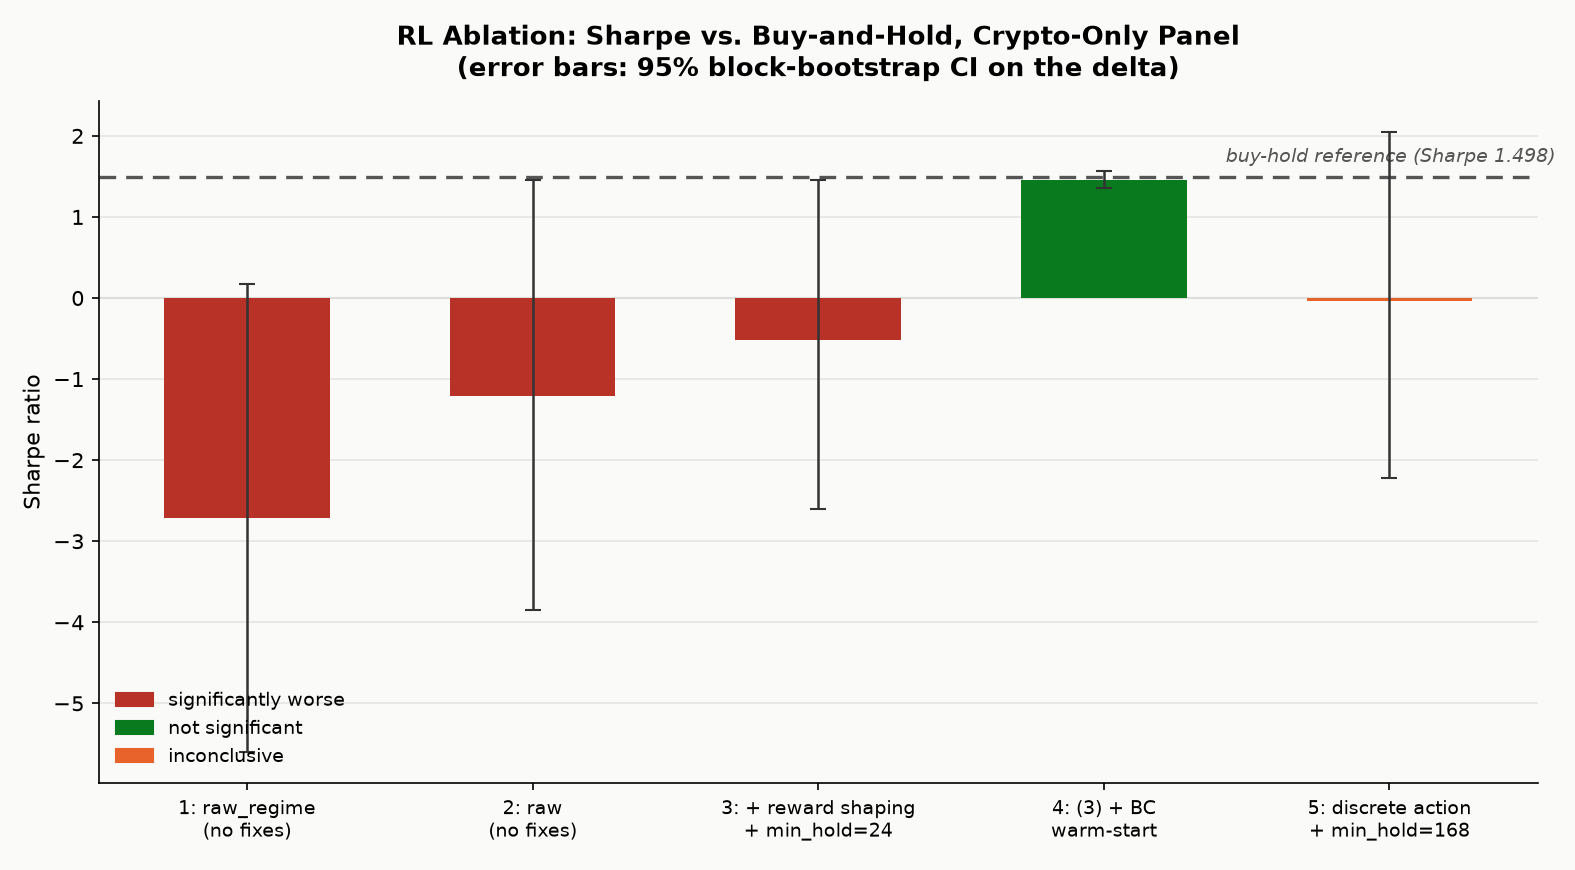
\includegraphics[width=0.85\textwidth]{images/rl_ablation_barplot.png}
    \caption{Absolute Sharpe ratio per ablation row against the buy-and-hold reference (dashed line, Sharpe 1.498). Error bars show the 95\% block-bootstrap confidence interval on the Sharpe delta, re-centered onto the absolute Sharpe axis; bar color follows the significance verdict of Table~\ref{tab:rl-ablation-crypto5}.}
    \label{fig:rl-ablation}
\end{figure}

Rows 1--2 isolate observation mode: dropping the regime-probability block improved Sharpe by roughly 1.5 points, consistent with a lookahead-bias defect identified independently (the HMM decode smooths over the entire concatenated sequence, so a regime probability at any training-split timestamp is influenced by data after it) --- but both configurations remained significantly worse than buy-and-hold, so removing the leaky feature alone was not sufficient. Row 3 isolates reward shaping: benchmark-relative reward plus a longer minimum hold narrowed the gap further without resolving it, and the policy was still trading almost as often (5{,}991 trades). Row 4, behavior-cloning warm-start from a buy-hold teacher, is the only configuration not significantly different from buy-and-hold --- but at only ten meaningful trades over a full year, and given a per-feature predictability check (Section~\ref{subsec:rl-ceiling-check}) finding only a modest directional edge exists at all, this result cannot be confirmed as a genuine edge over its own teacher rather than a faithful reproduction of it; both readings are consistent with the data at this sample size. Row 5 tested whether the continuous Beta position head itself was driving excess trading; it was not --- with a minimum hold seven times longer than row 3's, the discrete policy still traded roughly once every 8.5 days, almost exactly at the minimum-hold floor, and did not clear the pre-registered zero-Sharpe gate.

\subsection{Predictability Ceiling Check}
\label{subsec:rl-ceiling-check}

Before concluding the negative result reflects a structural limit rather than an unfound architecture, each of the crypto-panel's 22 features was tested alone (20 lags, ridge regression for magnitude $R^2$, logistic regression for direction, trained on data before 2024 and evaluated out-of-sample on 2024) against next-bar direction. Four of twenty-two features clear 52\% directional accuracy (\texttt{rsi} 54.3\%, \texttt{close\_return} 53.4\%, \texttt{obv\_raw} and \texttt{macd\_histogram} $\approx$53.1\%); $R^2$ for return magnitude is approximately zero or negative for every feature tested. This rules out ``there is genuinely nothing to find'' as a complete explanation --- row 4's behavior-cloning-preserved edge is not obviously impossible given a real, if weak, 54\% directional signal --- without confirming that the RL formulation is leaving value on the table either: the edge is real but small, and every architectural lever tested against it either made results worse or reproduced its teacher without demonstrably exceeding it.

\subsection{Final Decision on the RL Layer}
\label{subsec:rl-final-decision}

Following a stopping rule set before the final ablation row ran, specifically to avoid open-ended iteration against a fixed project timeline: rows 1, 2, 3, and 5 are each either significantly worse than buy-and-hold or statistically inconclusive, and row 4 cannot be confirmed as a genuine edge over its own teacher at ten trades. Four independent architectural levers --- regime conditioning, reward formulation, imitation warm-start, and action-space parameterization --- were each tested in isolation, and none produced a confirmed, statistically defensible improvement over buy-and-hold. This was adopted as the RL layer's result for the project, not a configuration still being searched over, with three consequences: the dashboard (Section~\ref{sec:dashboard-methodology}) ships with the multi-agent consensus and static execution path as its default signal source; RL execution remains available as an explicit, opt-in toggle carrying a warning about this section's finding; and this ablation table is reported as the project's controlled negative result on RL execution, evidenced end to end rather than asserted.

\subsection{Native Weekly-Decision-Cadence Follow-Up}
\label{subsec:rl-weekly-cadence}

The results above train the policy to re-decide every hour. A follow-up experiment tested whether forcing a full week's commitment per decision --- aggregating 168 hourly bars into a single decision, with the CVaR risk term scaled by $\sqrt{168}$ to remain comparable across horizons --- changed the outcome, motivated by the ceiling check above finding only a weak \emph{directional} edge that hourly rebalancing may be too fine-grained a horizon to extract.

Two engineering defects were found and corrected before any result from this experiment could be trusted: an annualization factor hardcoded for hourly returns, silently inflating an early result to an implausible Sharpe of 6.84 (a factor of $\sqrt{168}\approx13\times$, traced and fixed by threading the evaluation horizon explicitly through every metrics call site); and an evaluation script that reloaded the in-memory end-of-training model rather than the best-by-validation-Sharpe checkpoint every other evaluation path in the project uses, which for one configuration alone produced a fourfold difference in reported Sharpe. Both fixes were verified by independent hand reconciliation before any number from this experiment was trusted further.

With both fixes in place, a smoke test (two configurations, one seed each) cleared pre-registered thresholds set before the test ran (Sharpe 2.198 and 2.209 respectively), triggering a full grid of twelve independently trained runs: four observation conditions (raw features; raw features plus realized volatility; raw features plus regime probability; raw features plus a placebo-regime noise control) $\times$ three seeds each.

\begin{table}[H]
\centering
\small
\caption{Native weekly-cadence grid, BTC-only, validation year 2024. Sharpe recomputed with buy-and-hold aggregated to the identical weekly cadence (52 weekly observations); $\Delta$ from a block bootstrap (block size 4 weeks, 1000 resamples). Recomputed buy-hold reference: Sharpe 1.571. Full detail: \texttt{data/results/weekly\_grid\_reconciled.json}.}
\label{tab:rl-weekly-grid}
\begin{tabular}{|l|c|c|c|c|}
\hline
\textbf{Seed} & \textbf{A (raw)} & \textbf{B (raw+vol)} & \textbf{C (raw+regime)} & \textbf{D (raw+placebo)} \\
\hline
0 & 1.677 ($\Delta$+0.26) & 1.686 ($\Delta$+0.20) & 1.755 ($\Delta$+0.43) & 2.723 ($\Delta$+1.50) \\
\hline
1 & 1.688 ($\Delta$+0.31) & 1.883 ($\Delta$+0.45) & 1.665 ($\Delta$+0.40) & 1.764 ($\Delta$+0.57) \\
\hline
2 & 1.736 ($\Delta$+0.10) & 2.706 ($\Delta$+1.42) & 2.173 ($\Delta$+0.84) & 1.670 ($\Delta$+0.01) \\
\hline
\end{tabular}
\normalsize
\end{table}

\begin{figure}[!htbp]
    \centering
    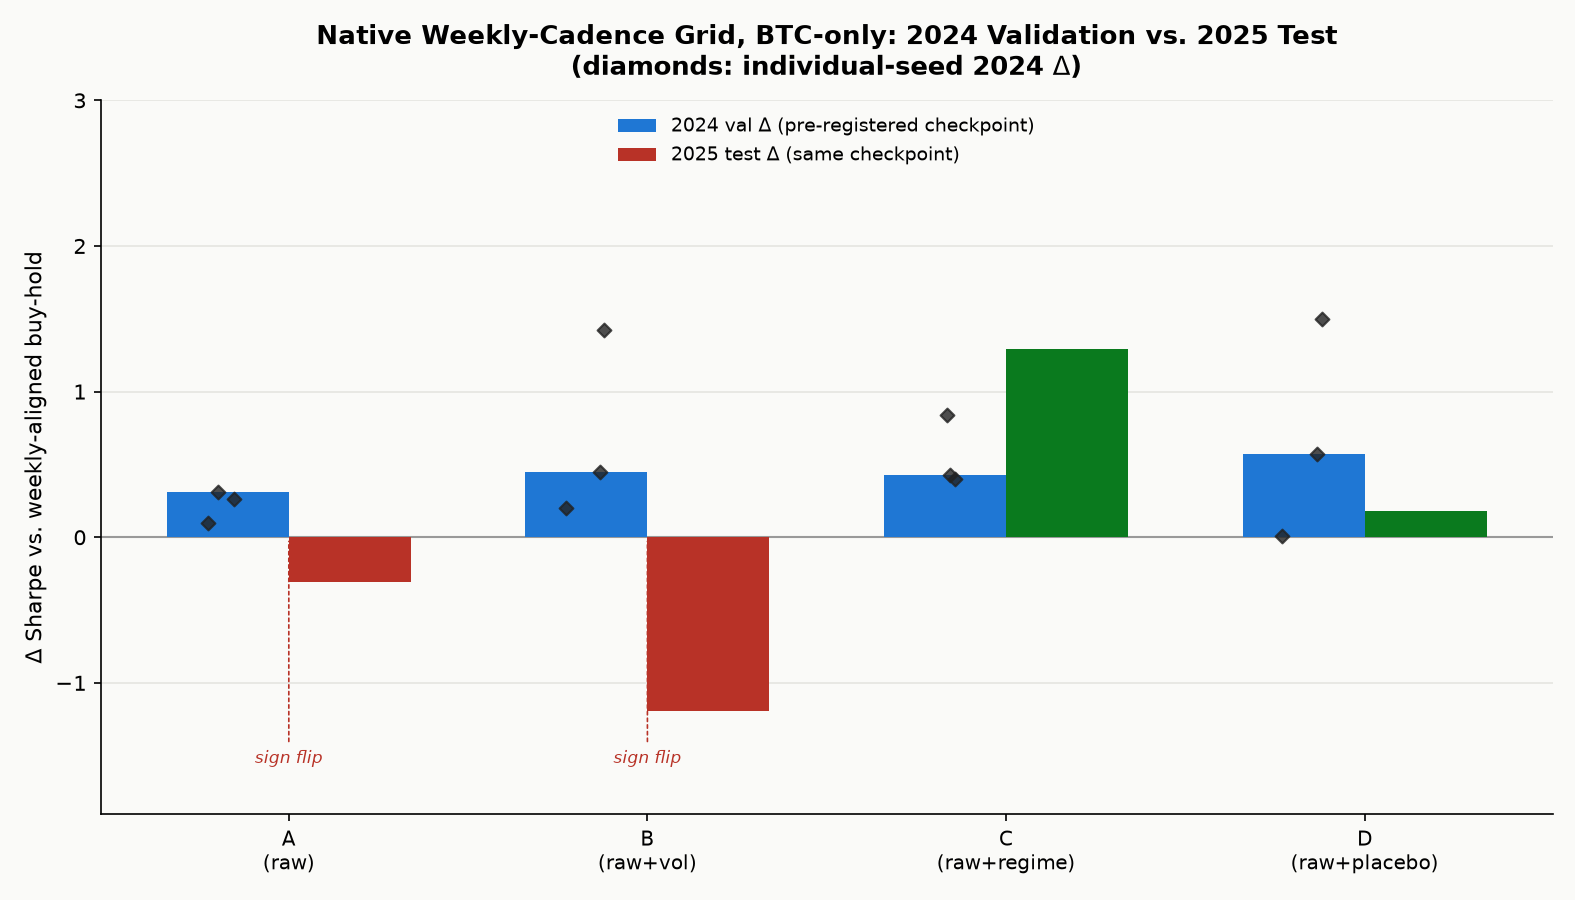
\includegraphics[width=0.85\textwidth]{images/weekly_grid_2024_2025_barplot.png}
    \caption{BTC-only weekly-cadence grid: the pre-registered checkpoint's $\Delta$ Sharpe vs.\ buy-hold on 2024 validation (blue) against the same checkpoint's $\Delta$ on 2025 test (red/green), from Table~\ref{tab:rl-weekly-2025}. Diamonds show the individual-seed 2024 $\Delta$ values of Table~\ref{tab:rl-weekly-grid} as context for the spread the pre-registered checkpoint was drawn from. Conditions A and B flip sign between the two years; C and D do not.}
    \label{fig:weekly-grid-2024-2025}
\end{figure}

None of the twelve 95\% confidence intervals excludes zero (widest, $[-1.93, 3.10]$; the narrowest still crosses it). Two things are simultaneously true and neither cancels the other: twelve of twelve independently trained runs beat buy-and-hold at the point estimate, which has not occurred for any prior configuration across this project's history; and zero of twelve individually reach significance, with confidence intervals this wide at only 52 weekly observations per validation pass. A naive sign-test argument over twelve independent trials does not apply here, because the trials are not independent in the sense that argument requires: all twelve runs are evaluated against the identical single 2024 market window, so consistent point-estimate wins are equally consistent with ``2024 favored a weekly-committed directional strategy generally'' as with any genuine, architecture-specific skill. Condition D, an explicit noise control carrying no real regime information, performs in the same range as condition C, the real regime condition --- consistent with every other regime-conditioning test in this chapter (Section~\ref{subsec:regime-downstream-value}) finding no measurable, noise-control-surviving value from regime conditioning.

On validation data alone, this is a directionally consistent but statistically unconfirmed lead; the out-of-window check below resolves it.

\subsubsection{2025 Test-Set Confirmation: the Lead Does Not Replicate}
\label{subsubsec:rl-weekly-2025}

Following this project's established test-set discipline, one checkpoint per condition was selected \emph{before} touching 2025 data, by median 2024 validation Sharpe among that condition's three seeds --- not best-of-three, which would already be a mild form of cherry-picking on the validation set (A$\to$seed~1, B$\to$seed~1, C$\to$seed~0, D$\to$seed~1). This selection was fixed in the evaluation script before it was ever run against 2025, and the script was run exactly once.

\begin{table}[H]
\centering
\small
\caption{2025 test-set pass, pre-registered checkpoints, one per condition. $\Delta$ vs.\ buy-hold; recomputed buy-hold weekly Sharpe on 2025 is $-0.291$ ($-15.9\%$ return), against $+1.571$ on 2024 --- a materially different market year.}
\label{tab:rl-weekly-2025}
\begin{tabular}{|l|c|c|c|c|}
\hline
 & \textbf{A (raw)} & \textbf{B (raw+vol)} & \textbf{C (raw+regime)} & \textbf{D (raw+placebo)} \\
\hline
2024 val $\Delta$ & +0.31 & +0.45 & +0.43 & +0.57 \\
\hline
\textbf{2025 test $\Delta$} & \textbf{--0.31} & \textbf{--1.19} & +1.29 & +0.18 \\
\hline
Significant? & no & no & no & no \\
\hline
\end{tabular}
\normalsize
\end{table}

Conditions A and B flipped sign entirely --- profitable relative to buy-hold in 2024, unprofitable relative to it in 2025 --- consistent with the 2024 result reflecting conditions favorable to any weekly-committed directional strategy that particular year, rather than a robust cadence-specific edge, exactly the risk raised when the validation grid was first reported (Section~\ref{subsec:rl-weekly-cadence}). Condition C is the one positive point estimate, and the largest delta of the four, but its 95\% CI is wide and crosses zero $[-1.709, 4.311]$, and a single pre-registered checkpoint on test cannot separate a genuine regime-conditioning benefit from that particular seed's idiosyncrasy. Condition D, the noise control, sits close to buy-hold and is not clearly separated from C either.

\textbf{This closes the investigation as not confirmed.} It does not overturn Section~\ref{subsec:rl-final-decision}'s final decision on the RL layer; it adds one further out-of-window data point consistent with it.

\subsubsection{Crypto5 Panel Extension: the Null Result Generalizes}
\label{subsubsec:rl-weekly-crypto5}

The BTC-only result above leaves one methodological concern unaddressed: 2024 was not equally favorable across assets (BTC bull, ETH mostly consolidating, BNB up on low volatility, LTC sideways-then-up, XRP up late), so a result benchmarked on BTC alone risks mistaking a favorable tailwind for genuine performance. This was tested directly by extending the same native-weekly-cadence design to the full crypto5 panel: a pilot grid (5 assets $\times$ the same 4 conditions, 1 seed each, 20 independently trained policies) reconciled with the identical weekly-aligned buy-hold and block-bootstrap methodology as the BTC-only result.

One consequential defect was found and fixed before trusting any cross-asset result: \texttt{evaluate\_ppo()}'s validation-environment builder silently defaulted to a hardcoded BTC-only asset list whenever a caller omitted an explicit one --- dormant until this point because every prior caller's configuration either was BTC-only or included BTC. Left uncaught, every non-BTC cell would have either evaluated a correctly-trained policy against BTC's own validation data or crashed outright, exactly the class of silent asset-mismatch defect this project has encountered more than once. Fixed by threading the configured asset list through both the validation-environment builder and the buy-hold baseline call, which carried the identical hardcoded default.

\textbf{2024 validation, reconciled:} 18 of 20 cells positive at the point estimate, but only \textbf{one of twenty reaches significance --- and it is condition D, the placebo/noise-control regime, not C, the real regime.} If regime conditioning carried genuine value, C should be the cell separating from noise; instead the opposite occurred on the one cell that cleared significance at all.

\textbf{Long-run diagnostic and 2025 out-of-window check, single pass per checkpoint, no re-runs:} each of the 20 checkpoints was walked continuously from 2024-01-01 through the last available bar (the crypto5 panel's aligned data ends 2025-12-31; a longer horizon is not reachable with this data), and the 2025-only portion of that same trajectory --- not a separate re-run --- was extracted as the out-of-window check.

\begin{table}[H]
\centering
\small
\caption{2025-only $\Delta$ vs.\ buy-hold, extracted from a single continuous 2024--2025 walk-forward pass per checkpoint, crypto5 panel, 1 seed. 0 of 20 cells significant.}
\label{tab:rl-weekly-crypto5-2025}
\begin{tabular}{|l|c|c|c|c|}
\hline
 & \textbf{A (raw)} & \textbf{B (raw+vol)} & \textbf{C (raw+regime)} & \textbf{D (raw+placebo)} \\
\hline
BTC & +1.27 & --0.46 & +0.15 & +0.60 \\
\hline
\textbf{ETH} & \textbf{--0.39} & \textbf{--0.43} & \textbf{--1.68} & \textbf{--0.35} \\
\hline
BNB & --0.89 & --1.18 & +0.65 & --1.30 \\
\hline
LTC & +0.55 & +0.86 & +0.22 & +0.57 \\
\hline
XRP & +2.41 & --0.08 & +0.01 & +1.18 \\
\hline
\end{tabular}
\normalsize
\end{table}

\begin{figure}[!htbp]
    \centering
    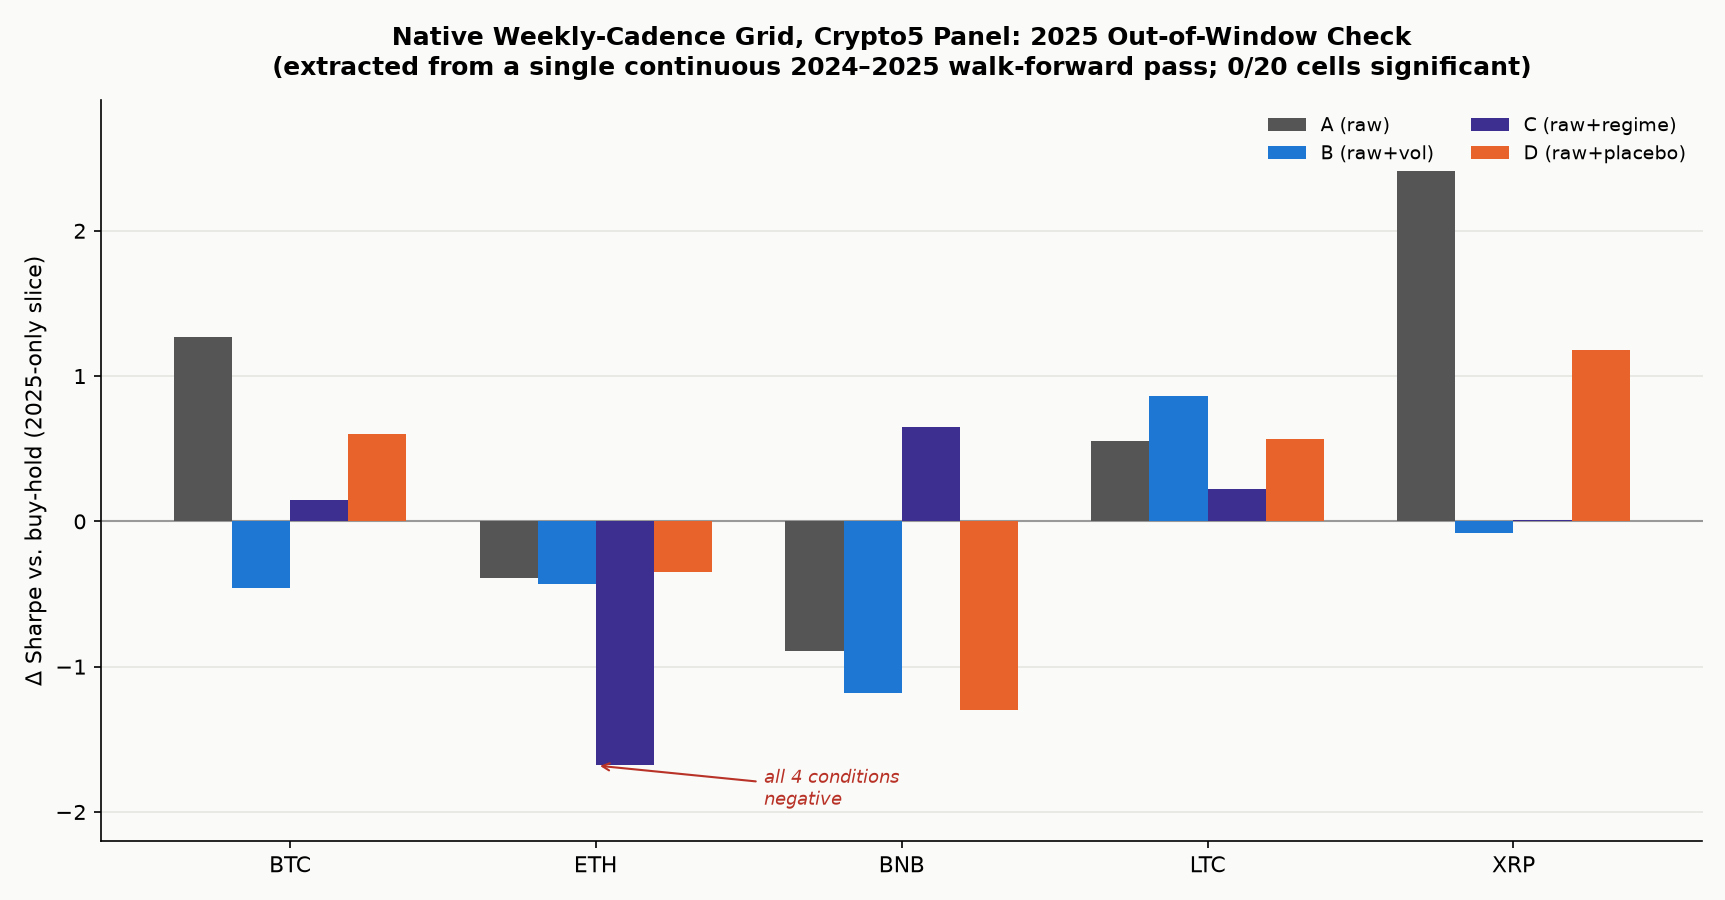
\includegraphics[width=\textwidth]{images/weekly_grid_crypto5_2025_barplot.png}
    \caption{Crypto5 panel extension, 2025-only $\Delta$ Sharpe vs.\ buy-hold per asset and condition (Table~\ref{tab:rl-weekly-crypto5-2025}). ETH is the one asset where all four conditions, including both the real regime condition (C) and its noise control (D), lose to buy-hold.}
    \label{fig:weekly-grid-crypto5-2025}
\end{figure}

The 2024 pattern (18/20 positive) weakens to 11/20 positive on the 2025 out-of-window check --- close to a coin flip --- and \textbf{ETH reverses completely: all four conditions lose to buy-hold in 2025}, having looked positive in the 2024 pilot. This is the identical favorable-year-artifact signature already found for BTC alone, now independently reproduced on a second asset. Condition C shows no separation from D on either split, on any asset.

Across the 20 cells of the 2025 out-of-window check, none reaches significance. To rule out that this single-seed pilot was simply unlucky, the grid was then completed to four seeds for every asset and condition (80 trained policies in total). Table~\ref{tab:rl-weekly-crypto5-4seed} reports the mean and standard deviation across seeds on 2024 validation.

\begin{table}[H]
\centering
\small
\caption{Weekly-cadence grid, crypto5 panel, 2024 validation Sharpe, mean $\pm$ standard deviation over four seeds.}
\label{tab:rl-weekly-crypto5-4seed}
\begin{tabular}{|l|c|c|c|c|}
\hline
 & \textbf{A (raw)} & \textbf{B (raw+vol)} & \textbf{C (raw+regime)} & \textbf{D (raw+placebo)} \\
\hline
BTC & $1.992 \pm 0.253$ & $2.055 \pm 0.643$ & $1.767 \pm 0.245$ & $2.353 \pm 0.247$ \\
\hline
ETH & $2.226 \pm 0.391$ & $2.553 \pm 0.119$ & $2.096 \pm 0.233$ & $2.146 \pm 0.259$ \\
\hline
BNB & $1.918 \pm 0.229$ & $2.216 \pm 0.616$ & $1.769 \pm 0.328$ & $1.805 \pm 0.166$ \\
\hline
LTC & $1.525 \pm 0.589$ & $1.557 \pm 0.778$ & $1.965 \pm 0.545$ & $1.289 \pm 0.795$ \\
\hline
XRP & $1.214 \pm 1.279$ & $2.054 \pm 0.488$ & $2.124 \pm 0.527$ & $2.093 \pm 0.265$ \\
\hline
\end{tabular}
\normalsize
\end{table}

The real-regime condition (C) does not separate from the placebo (D) on any asset: D's mean is higher than C's on BTC, BNB, and XRP, and the seed-to-seed standard deviations (0.12--1.28) are as large as or larger than the gaps between conditions. \textbf{Final verdict:} replicated on BTC alone, on the five-asset panel's 2024 validation with four seeds, and on the 2025 out-of-window check, the weekly-cadence result is consistent with every other regime-conditioning test in this project --- no measurable, noise-control-surviving benefit.
